% ---------------------------------------------------------------------------
% Pacific Graphics 2026 - 中文首版论文草稿
% ---------------------------------------------------------------------------
\documentclass{egpubl}
\usepackage{pg2026s}

\ConferenceSubmission

\usepackage{iftex}
\ifXeTeX
  \usepackage[UTF8]{ctex}
  \usepackage{graphicx}
\else
  \usepackage[T1]{fontenc}
  \usepackage{dfadobe}
  \usepackage{graphicx}
\fi

\biberVersion
\BibtexOrBiblatex
\usepackage[backend=biber,bibstyle=EG,citestyle=alphabetic,backref=true]{biblatex}
\addbibresource{references.bib}

\electronicVersion
\PrintedOrElectronic
\usepackage{egweblnk}

\usepackage{amsmath,amssymb,booktabs,multirow,array}
\usepackage[table]{xcolor}
\usepackage{algorithm}
\usepackage{algpseudocode}
\usepackage{enumitem}

\hypersetup{hidelinks}

\newcommand{\spags}{SPAGS}
\newcommand{\sps}{SPS}
\newcommand{\gap}{GAP}
\newcommand{\adm}{ADM}
\newcommand{\rtwo}{R\textsuperscript{2}-Gaussian}
\definecolor{rankone}{RGB}{190,32,32}
\definecolor{ranktwo}{RGB}{218,114,20}
\definecolor{rankthree}{RGB}{156,120,18}
\newcommand{\best}[1]{\textcolor{rankone}{\textbf{#1}}}
\newcommand{\second}[1]{\textcolor{ranktwo}{\textbf{#1}}}
\newcommand{\third}[1]{\textcolor{rankthree}{\textbf{#1}}}

\title{SPAGS: 面向稀疏视角 CT 新视图合成的空间感知渐进式自适应高斯泼溅}

\begin{document}
\maketitle

\begin{abstract}
稀疏视角 CT 新视图合成希望在极少投影下生成高质量的新角度 X 射线投影，从而减少辐射剂量并保留足够的结构信息。近年来，基于 3D Gaussian Splatting 的方法在效率上明显优于 NeRF，但现有方案仍存在三个关键缺口：其一，初始化通常缺乏解剖结构先验，导致重要区域欠覆盖、空白区域冗余；其二，面向自然场景设计的密化机制会在 CT 的高对比边界不断堆叠高斯，引发结构冗余；其三，密度参数的更新缺乏空间上下文，难以适应骨骼、软组织与空气之间明显不同的衰减分布。为此，我们提出 \spags，一个在初始化、密度控制与密度优化三个阶段显式引入空间感知的渐进式框架。具体而言，\sps\ 利用 FDK 重建提供的粗几何先验进行密度加权播种；\gap\ 在三维世界坐标系中依据邻近度与梯度活跃性联合剪除冗余高斯；\adm\ 通过 K-Planes 编码实现位置相关的密度调制。基于 5 个器官、2/3/4 视角设置的实验表明，\spags\ 在核心的 3-view 设定下取得 28.22 dB 的平均 PSNR，相比 \rtwo\ 提升 0.39 dB，并稳定优于 DN-Gaussian、CoR-GS、FSGS 与 X-Gaussian。该方法仅带来不到 10\% 的训练开销，不增加推理复杂度，适合作为稀疏视角 CT 新视图合成的高效基线。
\end{abstract}

\section{引言}
\label{sec:intro}

稀疏视角条件下的 CT 新视图合成（novel view synthesis, NVS）兼具明确的应用价值与突出的技术挑战。一方面，临床与工业场景希望通过减少采样视角来降低辐射剂量、缩短扫描时间并减轻设备负担；另一方面，视角稀缺会显著削弱几何约束，使得从少量 X 射线投影恢复稳定、连续且具有结构一致性的三维表示成为一个高度病态的问题。与自然图像中的新视图合成不同，X 射线成像遵循穿透式辐射传输，像素观测是整条射线路径上衰减累积的结果，因此其几何可辨识性、对初始化的敏感性以及对密度建模精度的依赖都更强~\cite{feldkamp1984practical,andersen1984simultaneous,wang2008image}.

近两年，3D Gaussian Splatting（3DGS）凭借显式表示与高并行栅格化，在新视图合成任务上展现出比 NeRF 更快的训练与渲染效率，并迅速扩展到结构化表示、抗锯齿渲染、网格提取、动态场景以及大尺度重建等方向~\cite{kerbl20233d,survey3dgs2024,scaffoldgs2024,mipsplatting2024,sugar2024,fourdgs2024,xu2024grid,wu2024deformable,lu2024compact}. 围绕稀疏视角场景，FSGS 借助邻近引导的高斯扩增来填补稀疏区域，并结合伪视角与深度先验约束几何结构~\cite{zhu2024fsgs}；CoR-GS 从双场协同的视角出发，用点分歧与渲染分歧来无监督识别重建不准确区域，再通过协同剪枝与协同正则化进行抑制~\cite{zhang2024cor}；DNGaussian 则进一步指出，当输入视角稀少时，高斯场的退化主要表现为几何错误，因此采用硬/软深度正则与全局-局部深度归一化来提升结构恢复能力~\cite{li2024dn}。与此同时，FreeNeRF、SparseNeRF 与 DepthSplat 等少样本神经渲染工作也从频率正则、深度排序与深度-高斯协同角度不断提高 sparse-view NVS 的上限~\cite{freenerf2023,sparsenerf2023,depthsplat2025}. 这些工作共同确立了一个重要趋势：在稀疏输入下，3DGS 的核心瓶颈不再只是渲染效率，而是如何稳定地约束几何与密度分布。

在 X 射线与 CT 场景中，这一问题进一步演化。X-Gaussian 首次系统性地将 3DGS 引入 X 射线新视图合成，通过辐射高斯点云模型、可微辐射栅格化与面向圆锥束扫描的均匀初始化，实现了比 NeRF 快得多的投影生成~\cite{cai2024xgaussian}。随后，\rtwo\ 进一步从体重建角度揭示出标准 3DGS 在 X 射线任务中的积分偏差问题，并通过新的 radiative kernel、X 射线栅格化与可微体素化，建立了首个面向稀疏视角断层重建的 3DGS 框架~\cite{hu2024r2}。最近，X$^2$-Gaussian 又把 radiative Gaussian 扩展到连续时间 4D CT，而 GR-Gaussian 则从图结构梯度建模的角度缓解极稀疏条件下的针状伪影~\cite{x2gaussian2025,grgaussian2025}。然而，从我们的实验与误差分析来看，现有 CT 场景中的 3DGS 方案仍主要解决了“能否用于 X 射线渲染”和“如何修正积分偏差”的问题，却尚未充分回答另一个更贴近优化过程本身的问题：当观察视角极少时，三维高斯该如何在空间中被初始化、增删和调制，才能真正适配 CT 解剖结构的分布规律？

我们的核心观察是：对于稀疏视角 CT 新视图合成，主要矛盾并不只是“空间不够稀疏”，而是“结构冗余被错误地放大”。在自然场景中，FSGS 一类方法通过向高斯稀疏区域补点来改善覆盖不足，这与前向 RGB 场景“大片空间为空、可见表面稀疏”的事实是匹配的~\cite{zhu2024fsgs}。但 CT 体数据并非由前景表面和空背景组成，而是一个整体被不同组织密度连续占据的体空间：骨组织与软组织边界处往往拥有最强的梯度信号，于是传统的“梯度越大越加点”策略会持续在边界堆叠高斯，导致表示容量被冗余消耗；而组织内部与低对比区域反而得不到足够稳定的密度建模。换句话说，CT 中真正需要解决的往往不是 coverage gap，而是 redundancy control。

基于这一认识，我们提出 \spags，一个面向稀疏视角 CT 新视图合成的空间感知渐进式自适应高斯泼溅框架。其设计遵循一个统一原则：在 3DGS 的关键决策点显式引入空间先验，而不是完全依赖局部梯度信号自行演化。首先，在初始化阶段，我们利用 FDK 重建得到的粗体密度图作为空间先验，提出 \sps（Spatial Prior Seeding），通过“密度加权采样 + 均匀补偿采样”的混合播种方式，让高斯从一开始就更多落在解剖相关区域。其次，在训练中的密度控制阶段，我们提出 \gap（Geometry-aware Pruning），不再沿用自然图像任务中“向稀疏区域补高斯”的思路，而是在三维世界坐标系下对局部过度聚集的高斯进行邻近度评估，并结合梯度活跃性过滤，仅剪除那些既拥挤又不再有效学习的冗余高斯。最后，在密度优化阶段，我们提出 \adm（Adaptive Density Modulation），通过 K-Planes 编码与轻量解码器学习位置相关的密度修正，使不同解剖区域能够拥有不同的密度调节规律。

与现有五个核心对比方法相比，我们的定位是明确而互补的。FSGS 更强调通过 proximity-guided unpooling 扩张稀疏高斯覆盖~\cite{zhu2024fsgs}；CoR-GS 借由双场分歧来抑制不一致几何~\cite{zhang2024cor}；DNGaussian 聚焦于用外部深度先验修复稀疏视角下的几何退化~\cite{li2024dn}；X-Gaussian 改造了 X 射线成像条件下的高斯表示与初始化方式~\cite{cai2024xgaussian}；\rtwo\ 则从体重建角度修复了 3DGS 的积分偏差并提供可微体素化能力~\cite{hu2024r2}。而 \spags\ 的关注点是进一步向前推进一步：在已经具备辐射渲染基础之后，如何让高斯的空间分布与密度更新机制真正适配 CT 体数据的结构规律。图~\ref{fig:intro-compare} 从抽象 pipeline 层面对比了本文与主流 sparse-view 3DGS 方法的差异。

\begin{figure}[t]
\centering
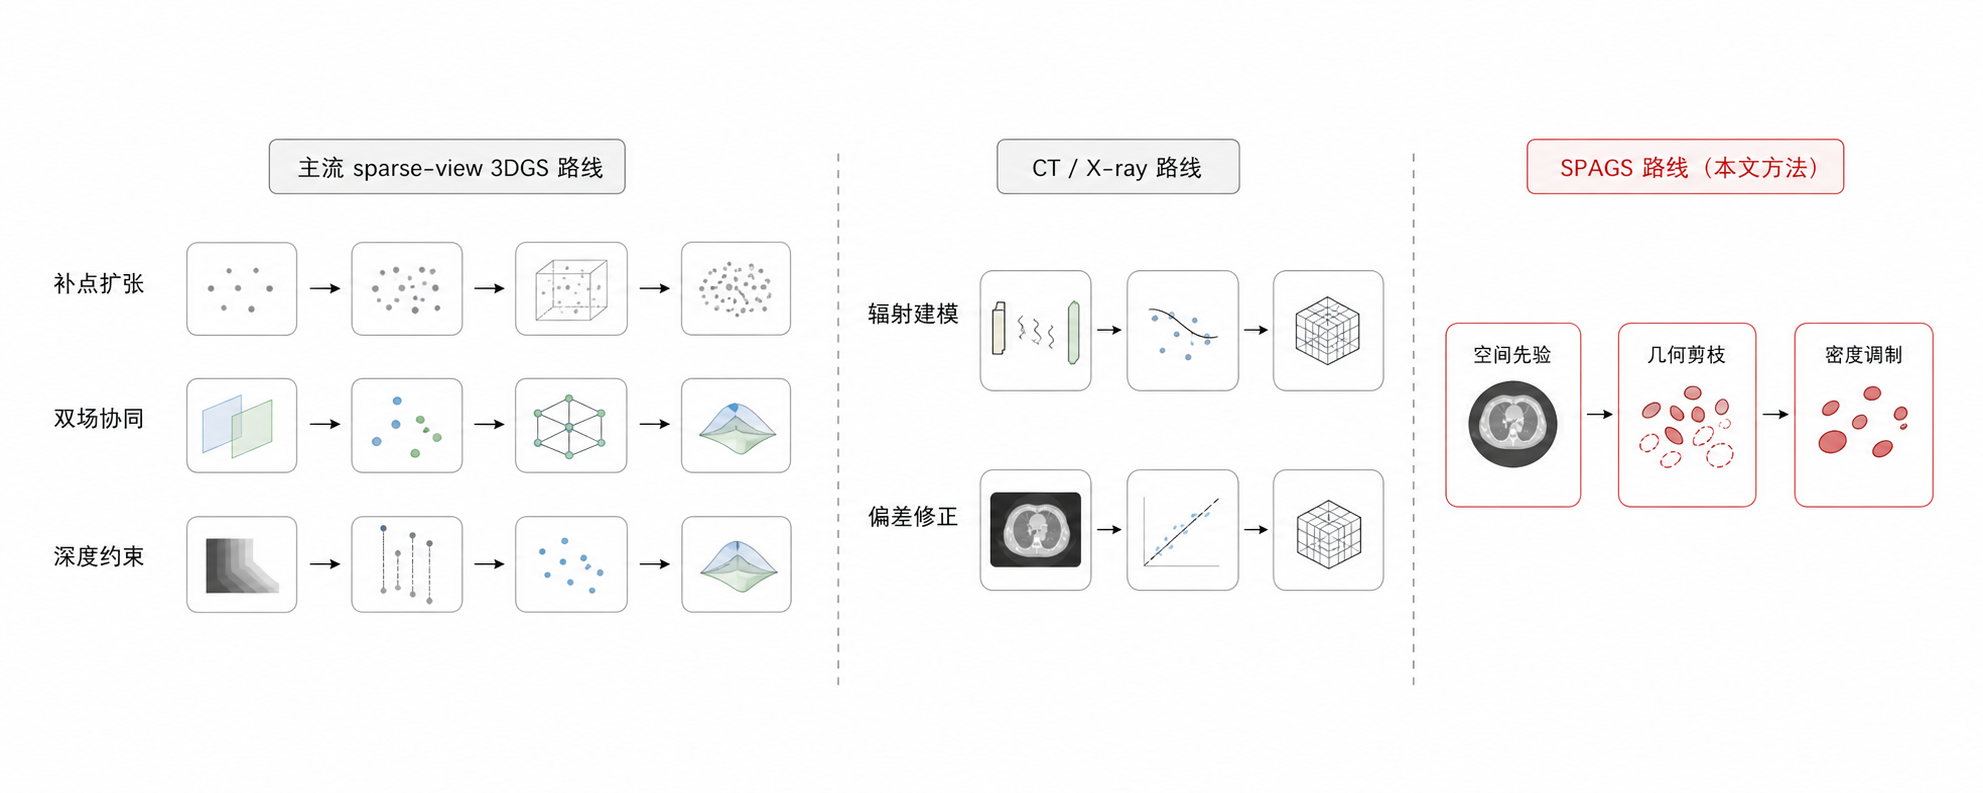
\includegraphics[width=\linewidth]{figures/fig_intro_compare.png}
\caption{与主流 sparse-view 3DGS 路线的抽象对比。本文方法在初始化、冗余控制与密度更新三个阶段都显式引入了空间感知。}
\label{fig:intro-compare}
\end{figure}

我们的贡献可以概括为三点：
\begin{itemize}[leftmargin=1.5em]
  \item 我们提出 \sps，利用 FDK 粗重建提供的体密度先验进行空间感知播种，从初始化阶段减少空区域冗余并提升解剖相关区域覆盖。
  \item 我们提出 \gap，在三维世界坐标中基于邻近度与梯度活跃性联合剪除冗余高斯，直接针对稀疏视角 CT 中的结构冗余问题。
  \item 我们提出 \adm，通过 K-Planes 实现位置相关的密度调制，使高斯密度更新能够响应骨骼、软组织与空气等不同区域的空间异质性。
\end{itemize}

在 5 个器官、2/3/4 视角的设置下，\spags\ 在核心 3-view 设定中达到 28.22 dB 平均 PSNR，相比 \rtwo\ 提升 0.39 dB，并在大多数器官与视角上优于其余对比方法。更重要的是，消融实验显示 \gap\ 带来的冗余控制收益最为稳定，验证了我们的中心判断：对于稀疏视角 CT 任务，显式的空间感知与结构冗余控制，是比单纯补点更关键的优化方向。

\section{相关工作}
\label{sec:related}

\subsection{稀疏视角 3D Gaussian Splatting}

3D Gaussian Splatting 通过一组三维各向异性高斯显式表示场景，并依赖可微分栅格化实现高效渲染，在效率与质量之间取得了优于传统 NeRF 的平衡~\cite{kerbl20233d}。自 2023 年提出以来，围绕 3DGS 的工作迅速扩展到大尺度场景、视角自适应结构化表示、抗锯齿渲染、显式网格提取、动态时空建模与紧凑表示压缩等方向~\cite{survey3dgs2024,scaffoldgs2024,mipsplatting2024,sugar2024,fourdgs2024,xu2024grid,wu2024deformable,lu2024compact,roessle2024densification}。在密集视角条件下，这类方法已经广泛用于表面重建、动态场景建模与各类三维生成任务；但当输入视角显著减少时，3DGS 容易暴露几何不稳定、密化失真与过拟合等问题，因此“如何让 3DGS 适配 sparse-view setting”成为近一阶段的重要研究主线~\cite{zhang2024cor,li2024dn,zhu2024fsgs}.

FSGS 的写法非常典型地体现了这一方向的第一类思路：把问题理解为“稀疏初始化导致场景覆盖不足”，然后在原始 3DGS 的 densification 流程上引入 proximity-guided Gaussian unpooling，在已有高斯之间生成新的高斯，以提高表示密度并填补空洞区域~\cite{zhu2024fsgs}。同时，FSGS 还通过伪视角与单目深度先验来约束训练过程，避免有限视角下的过拟合。对自然 RGB 场景而言，这一设计非常合理，因为场景的几何支撑主要集中在可见表面，真实困难在于“表面之间有较大空隙、初始 SfM 点不够密”。

CoR-GS 代表了第二类思路：与其单独优化一个高斯场，不如并行优化两个随机初始化但共享监督的高斯场，并把二者在点位置与渲染结果上的分歧当作重建质量的无监督信号~\cite{zhang2024cor}。基于这一观察，CoR-GS 设计了 co-pruning 与 pseudo-view co-regularization，用以压制不一致几何与不稳定渲染。该方法的重要启发在于，它将“稀疏视角下的不确定性”显式转化成可观测的 disagreement，并将其纳入优化目标。

DNGaussian 则更接近第三类思路：把 sparse-view 3DGS 的主要退化归因于几何错误，因此从深度监督角度进行修复~\cite{li2024dn}。该方法提出 Hard and Soft Depth Regularization 以及 Global-Local Depth Normalization，在保持显式高斯渲染效率的同时，引入单目深度先验来校正几何结构，并特别强调对局部细粒度深度变化的响应能力。与 FSGS、CoR-GS 相比，DNGaussian 更直接地把“几何恢复”置于问题核心。

这些方法共同推动了 sparse-view 3DGS 的进展，但其隐含前提仍主要来自自然图像场景：观察对象由表面主导，视角约束不足时最关键的是如何补足几何、减少漂浮点、压制外部监督带来的噪声。与这些基于优化的方法并行，近期也有一批方法从前馈或泛化重建角度探索少视图高斯表示，例如围绕深度协同与多视图先验的工作不断出现~\cite{chen2022pixelnerf,freenerf2023,sparsenerf2023,depthsplat2025}. 然而在 CT 场景中，三维空间是被体密度连续占据的，问题不再只是“几何不准”或“表面覆盖不够”，而是高斯会在高对比边界被反复密化并形成结构冗余。我们的工作正是在这一差异之上，与 FSGS、CoR-GS、DNGaussian 拉开问题设定上的边界。

\subsection{X 射线新视图合成与 CT 断层重建}

传统 CT 重建方法大体可以分为解析法与迭代法。以 FDK 为代表的解析方法依赖滤波反投影，计算效率高，但在稀疏视角下容易产生条纹伪影；SART 等迭代方法能够更稳健地引入先验约束，但计算成本较高~\cite{feldkamp1984practical,andersen1984simultaneous}. 随着神经场方法的发展，越来越多工作开始用坐标网络建模体密度场，并通过自监督投影重建来进行病例级优化~\cite{mildenhall2021nerf,zha2023nerfsurvey,guan2024naf,shen2024saxnerf}. 虽然这类方法在表示能力上表现强劲，但由于体渲染依赖海量点采样，训练与推理开销通常难以满足高效应用场景的需求；为缓解这一问题，Instant-NGP、TensoRF 等高效表示也提供了启发~\cite{muller2022instant,chen2022tensorf}.

X-Gaussian 首次较为系统地把 3DGS 引入 X 射线新视图合成。与自然图像不同，X 射线投影满足穿透式成像而非表面反射，因此 X-Gaussian 重新定义了 radiative Gaussian point cloud，并提出可微辐射栅格化（Differentiable Radiative Rasterization）以及面向圆锥束扫描的 ACUI 初始化策略，从而显著提升了 X 射线 NVS 的训练与推理效率~\cite{cai2024xgaussian}. 这项工作的意义在于说明：3DGS 并非只能服务于 RGB 场景，只要渲染物理被正确改写，它同样可以成为 X 射线任务中的高效表示。随后，X$^2$-Gaussian 把 radiative Gaussian 表示推进到连续时间 4D CT，而 GR-Gaussian 从图结构梯度建模的角度进一步缓解针状伪影，说明 CT-3DGS 已经开始从“可用”走向“细化优化”阶段~\cite{x2gaussian2025,grgaussian2025}。

\rtwo\ 则向前推进到“直接体重建”的层面。该工作指出标准 3DGS 在从三维高斯投影到二维高斯的过程中存在积分偏差，这一偏差对普通图像渲染影响有限，但会严重破坏体密度恢复的一致性~\cite{hu2024r2}. 因此，\rtwo\ 通过新的 radiative kernel、X 射线栅格化与可微体素化，把 3DGS 真正扩展为可用于稀疏视角断层重建的框架。换言之，X-Gaussian 主要解决“如何高效合成 X 射线投影”，而 \rtwo\ 进一步解决“如何准确恢复体密度场”。

从我们的角度看，X-Gaussian 与 \rtwo\ 已经搭好了 CT 领域 3DGS 的物理基础与渲染基础，但在优化层面仍保留了较多来自通用 3DGS 的默认假设。例如，初始化虽然已不再依赖 SfM，但仍缺乏对具体解剖复杂度的自适应分配；密度控制虽然可以借助梯度进行克隆与分裂，但并未显式约束边界区域的冗余堆叠；密度参数本身也仍主要依赖逐点梯度更新，而缺少连续空间上下文。因此，我们将 \spags\ 的定位放在“继承 CT-3DGS 物理正确性之后，补足其空间分布建模能力”这一层面。

\subsection{我们与五个核心对比方法的关系}

由于本文的对比方法恰好覆盖了 sparse-view 3DGS 与 X-ray/CT 3DGS 的两个关键谱系，因此它们也构成了定位 \spags\ 的最直接坐标系。FSGS 将 sparse-view 问题理解为“高斯不够、覆盖不足”，其方法论是补点与扩张；CoR-GS 将问题理解为“单场优化不稳定”，其方法论是通过双场 disagreement 进行无监督纠偏；DNGaussian 将问题理解为“几何在稀疏视角下退化”，其方法论是深度先验与归一化约束；X-Gaussian 将问题理解为“自然图像版 3DGS 不适合 X 射线物理”，其方法论是辐射建模与 scanner-aware 初始化；\rtwo\ 则进一步将问题锚定为“3DGS 在体重建场景中存在积分偏差”，并通过 kernel、rasterization 与 voxelization 做出系统修正~\cite{zhu2024fsgs,zhang2024cor,li2024dn,cai2024xgaussian,hu2024r2}.

与这些方法相比，\spags\ 的新意并不在于重新定义 X 射线成像物理，也不在于依赖额外大模型或双场结构，而在于提出一个更贴合 CT 体空间分布规律的优化观点：在极稀疏视角下，问题的主导项往往是结构冗余而非单纯稀疏，因而初始化、剪枝与密度调制都应该围绕“空间感知”展开。基于这一判断，我们提出的 \sps/\gap/\adm\ 分别对应空间感知初始化、空间感知冗余控制与空间感知密度修正，从而与上述五类代表工作形成互补而清晰的差异化路线。

\section{方法}
\label{sec:method}

我们将稀疏视角 CT 新视图合成拆分为三个彼此衔接的子问题：如何让初始高斯尽量落在有意义的解剖区域、如何在训练过程中抑制边界区域的冗余堆叠、以及如何让密度更新显式响应空间上下文。围绕这三个问题，我们提出 \spags\ 的三阶段框架，如图~\ref{fig:pipeline} 所示。

\begin{figure}[t]
\centering
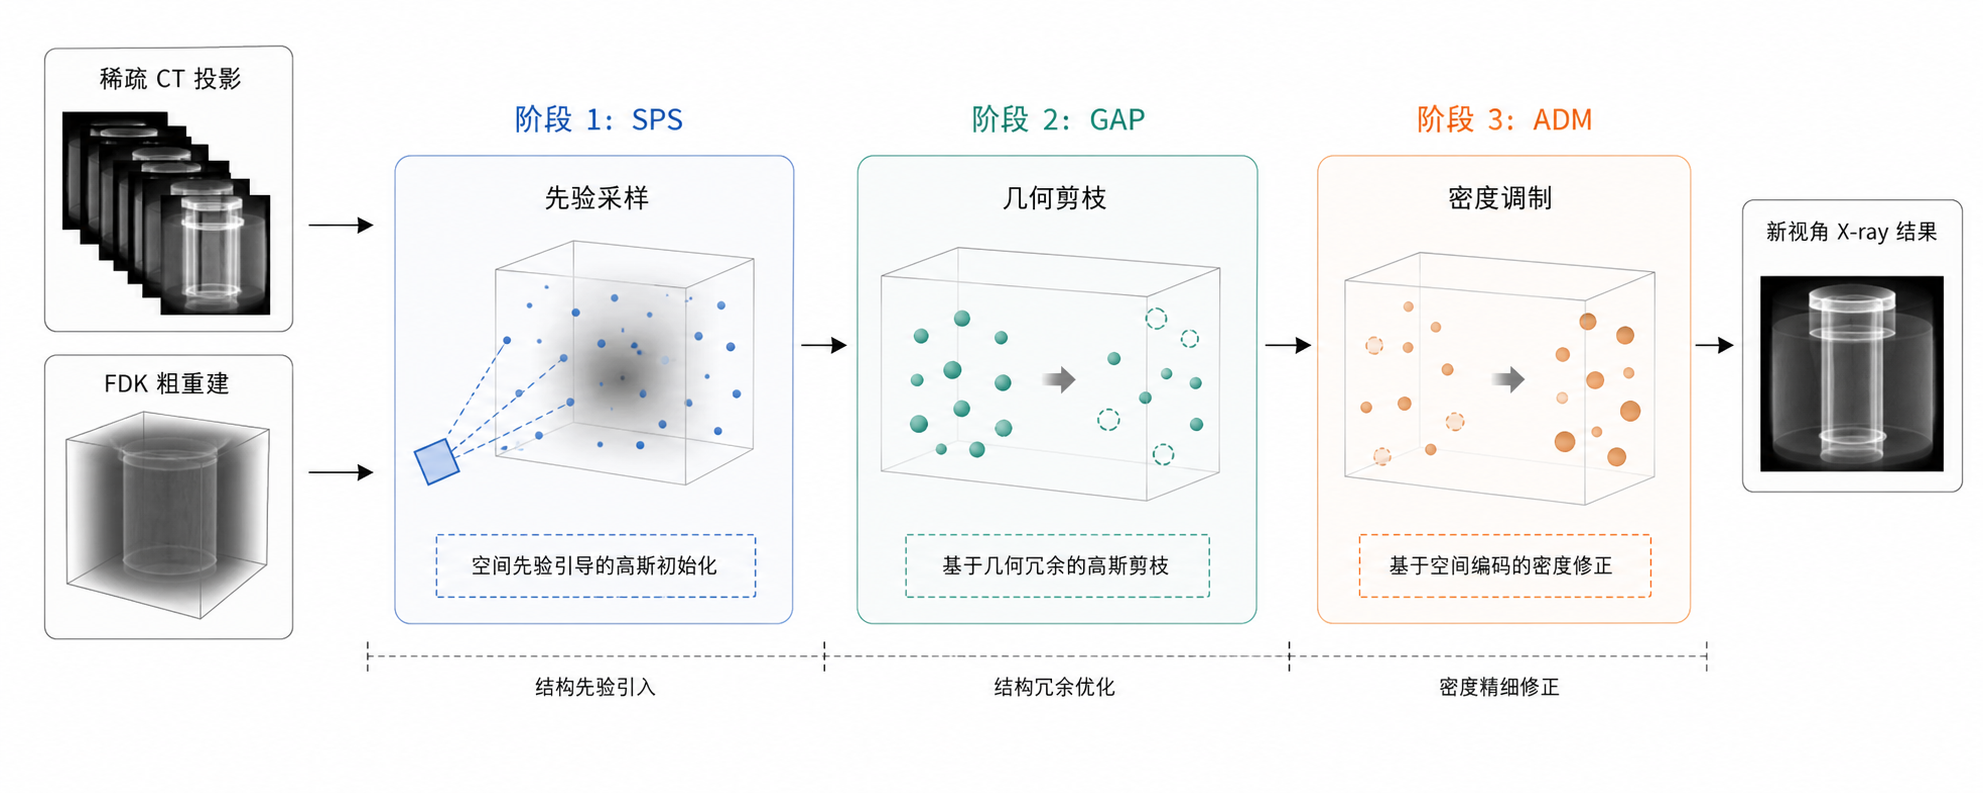
\includegraphics[width=\linewidth]{figures/fig_pipeline.png}
\caption{\spags\ 的总体流程。输入稀疏投影与 FDK 粗重建，经 \sps、\gap\ 与 \adm\ 三阶段逐步收紧高斯空间分布，输出目标新视角 X-ray。}
\label{fig:pipeline}
\end{figure}

\subsection{阶段一：Spatial Prior Seeding（\sps）}

在极少视角条件下，初始化的好坏会显著影响后续优化轨迹。标准 3DGS 往往采用均匀采样或依赖 SfM 点云初始化，但这两种方式都不适合 CT 场景：前者无法区分空气、软组织与骨骼的解剖重要性，后者则因为 X 射线投影的灰度重叠与低纹理特征难以稳定工作~\cite{cai2024xgaussian}. 我们因此使用 FDK 重建产生的粗体密度图 $V_{\text{FDK}}$ 作为空间先验，对初始高斯进行密度加权采样：
\begin{equation}
p(\mathbf{x}) \propto \max(V_{\text{FDK}}(\mathbf{x}), \epsilon)^\gamma,
\end{equation}
其中 $\epsilon$ 用于避免背景区域出现零概率，$\gamma$ 控制采样集中度。

仅靠密度加权会使高斯过度聚集在亮度最高的骨性结构附近，因此我们引入混合采样：
\begin{equation}
\mathbf{X} = \mathbf{X}_{\text{uniform}} \cup \mathbf{X}_{\text{weighted}},
\end{equation}
其中 20\% 的点来自均匀采样，80\% 的点来自密度加权采样。这样既能保证整体覆盖，又能让更多高斯优先分配给解剖复杂区域。采样位置确定后，我们将 FDK 值作为初始密度，并根据局部采样密度设定尺度参数，最终得到 50K 个初始高斯。

\begin{figure}[t]
\centering
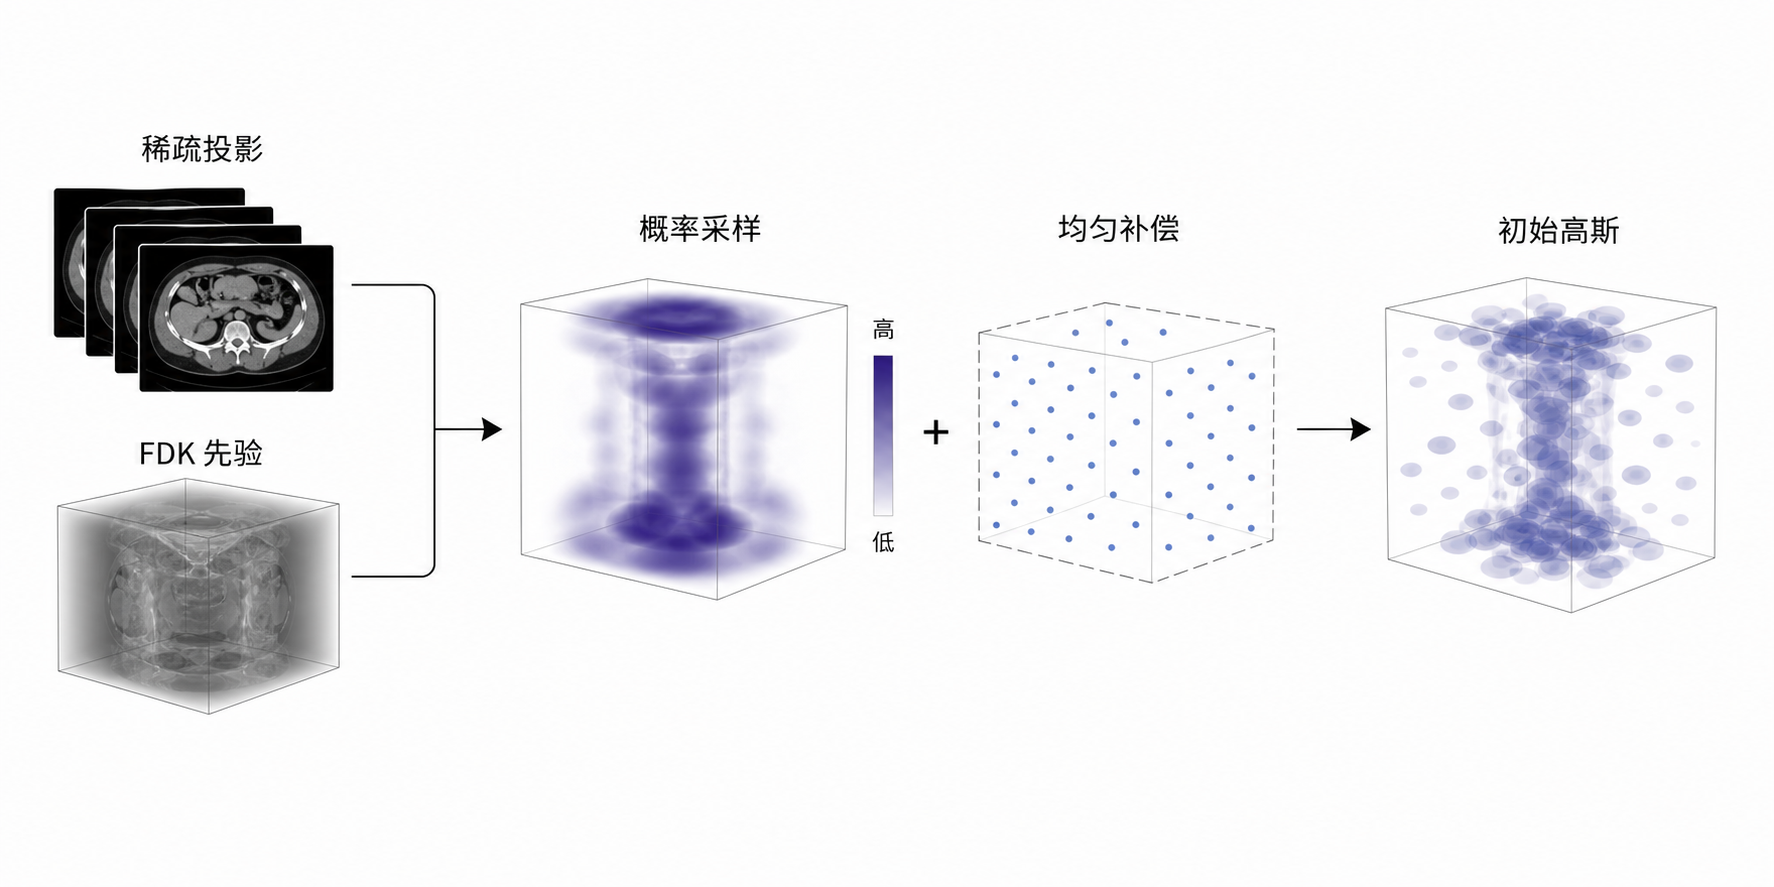
\includegraphics[width=\linewidth]{figures/fig_sps.png}
\caption{\sps\ 模块示意。利用 FDK 粗重建引导密度加权采样，并用少量均匀补偿保证全局覆盖。}
\label{fig:sps}
\end{figure}

\subsection{阶段二：Geometry-aware Pruning（\gap）}

在 CT 场景中，传统基于梯度的 densification 往往会在骨组织与软组织边界持续复制高斯，因为这些区域的投影误差梯度最大。问题在于，这类高梯度不一定意味着“覆盖不足”，也可能只是“同一结构被过多高斯竞争表示”。因此，我们不沿用 FSGS 那种面向稀疏区域补点的思路~\cite{zhu2024fsgs}，而是直接在世界坐标系中度量局部拥挤程度。

具体来说，对每个高斯 $G_i$，我们计算其与 $K$ 个最近邻的平均欧氏距离作为邻近度评分：
\begin{equation}
s(\mathbf{p}_i)=\frac{1}{K}\sum_{j=1}^{K}\|\mathbf{p}_i-\mathbf{p}_j\|_2.
\end{equation}
当 $s(\mathbf{p}_i)$ 低于阈值 $\tau$ 时，说明该高斯处于过度聚集区域。为了避免误删仍在有效学习的高斯，我们再引入梯度活跃性过滤：只有当其累积位置梯度低于阈值 $\delta$ 时，才将其视为真正的冗余候选。最终，每轮最多剪除总高斯数的 2\%，并在第 2K 到 20K 次迭代间每 500 次触发一次。

\begin{figure}[t]
\centering
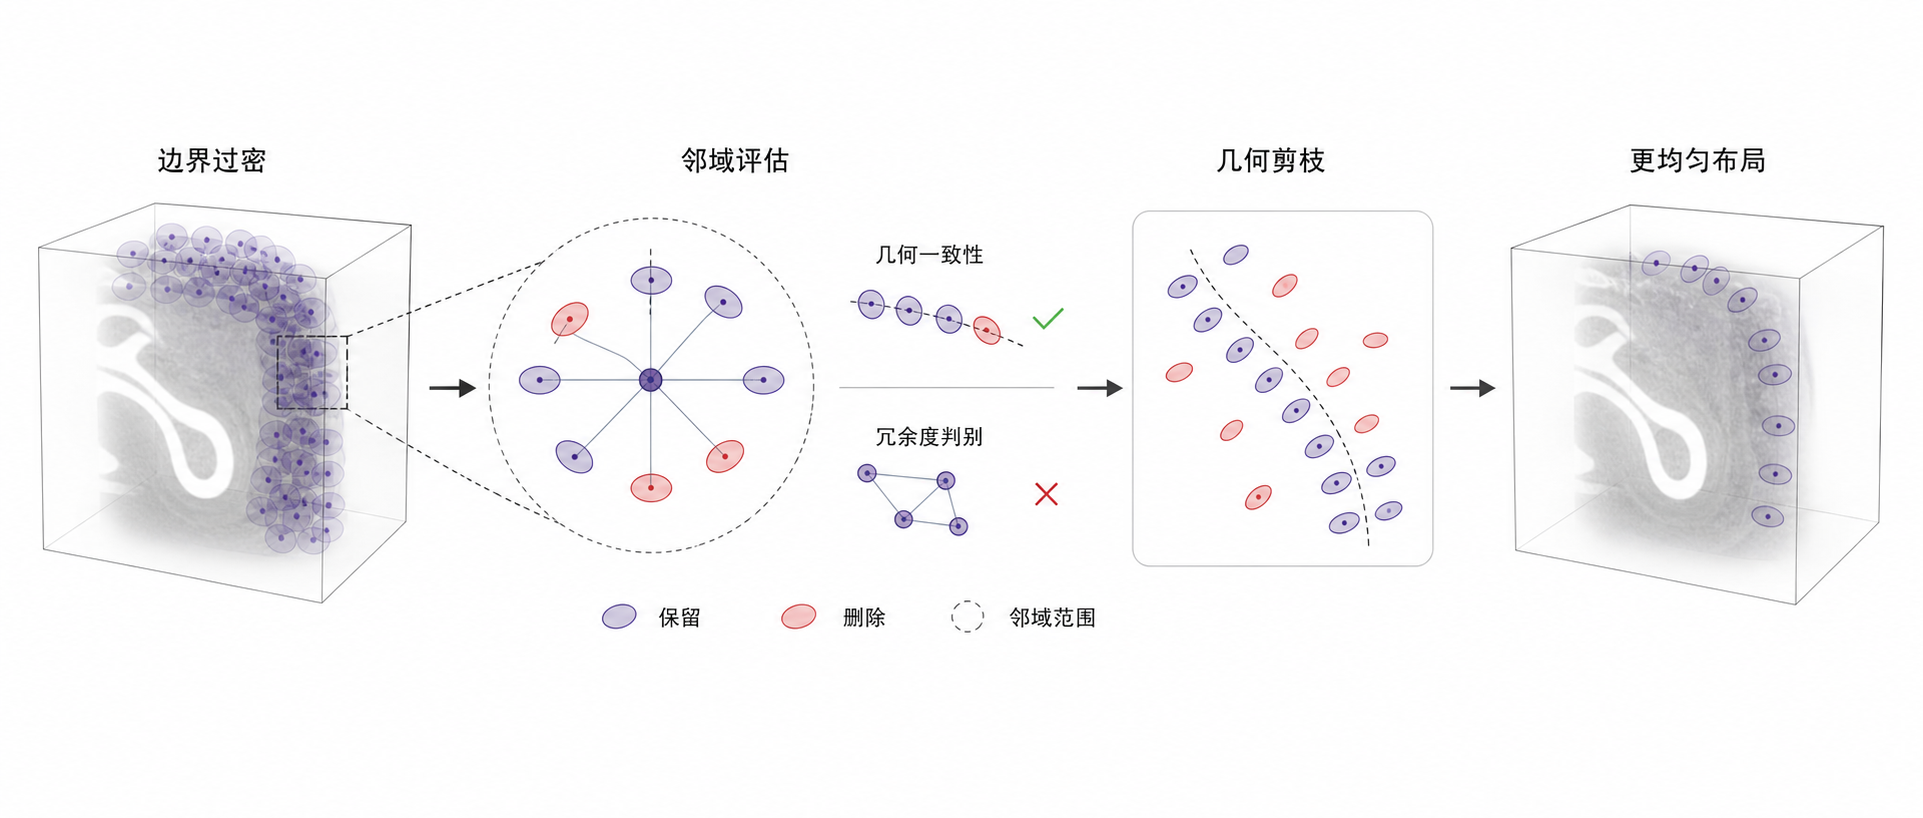
\includegraphics[width=\linewidth]{figures/fig_gap.png}
\caption{\gap\ 模块示意。依据三维邻近度与梯度活跃性联合识别并剪除边界附近的冗余高斯。}
\label{fig:gap}
\end{figure}

这一步的关键不在“减少高斯数量”本身，而在建立一种负反馈机制：当标准 3DGS 的密化策略在边界附近过度扩张时，\gap\ 能及时把冗余点回收，使表示容量回到真正需要的位置。我们的消融实验也证实，\gap\ 是三者中收益最稳定、幅度最大的模块。

\subsection{阶段三：Adaptive Density Modulation（\adm）}

即便有了更合理的初始化与冗余控制，不同解剖区域的密度更新规律仍然并不相同。骨组织应具有更高衰减系数，肺部空气区域应保持更低密度，而软组织往往需要平滑过渡。如果所有高斯都依赖相同的逐点梯度更新，模型会难以学到这种空间异质性。为此，我们引入 \adm，用 K-Planes 对高斯中心位置进行编码，并通过轻量解码器预测位置相关的密度偏移与置信度。

给定位置 $\mathbf{x}$，我们从三组正交平面特征中采样并拼接成空间编码 $F(\mathbf{x})$。这种 K-Planes 编码最早被用于显式时空辐射场建模，能够以较低成本提供连续空间上下文~\cite{fridovich2022kplanes}。在此基础上，我们用 MLP 输出密度偏移 $\Delta \rho(\mathbf{x})$ 和置信度 $c(\mathbf{x})$，最终写成：
\begin{equation}
\rho_{\text{final}}(\mathbf{x})=\rho_{\text{base}}(\mathbf{x})+c(\mathbf{x})\cdot\Delta\rho(\mathbf{x}).
\end{equation}
为了避免引入全局偏置，我们对偏移量进行零均值归一化，使 \adm\ 更专注于学习局部相对修正，而非整体抬升或压低全部密度。

\begin{figure}[t]
\centering
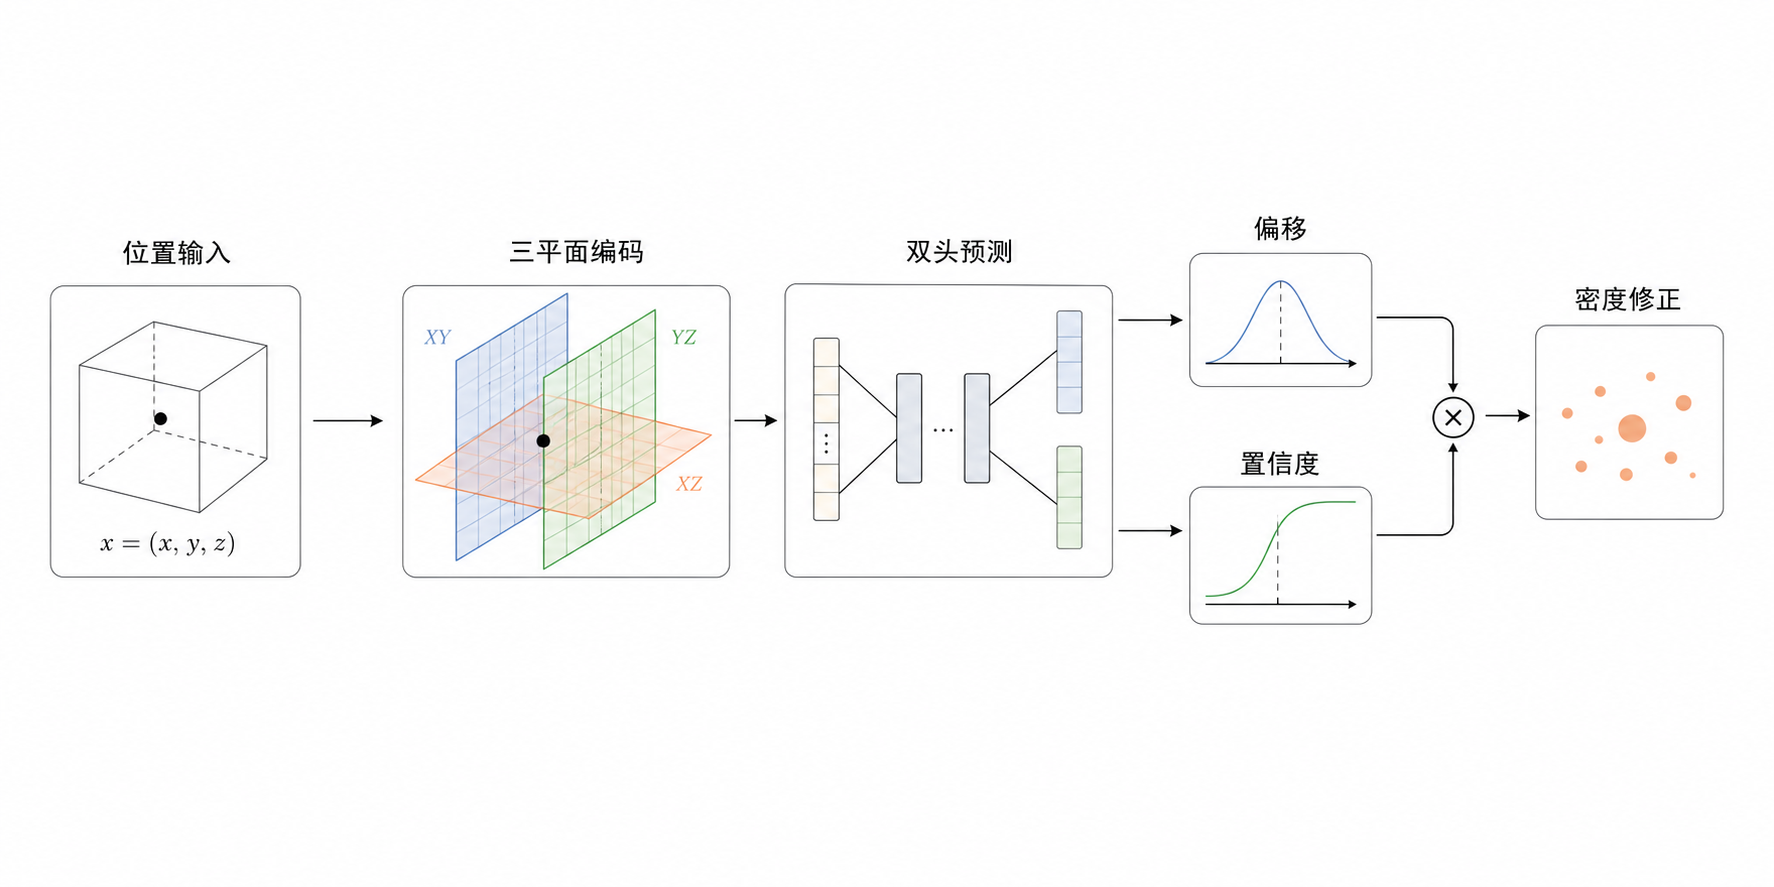
\includegraphics[width=\linewidth]{figures/fig_adm.png}
\caption{\adm\ 模块示意。基于 K-Planes 空间编码预测密度偏移与置信度，实现位置相关的密度调制。}
\label{fig:adm}
\end{figure}

\subsection{整体训练流程}

\spags\ 的三阶段并非彼此独立，而是形成一个逐步收紧空间结构的优化链路：\sps\ 决定“高斯从哪里开始”，\gap\ 决定“哪些高斯不该继续留着”，\adm\ 决定“留下来的高斯应如何因地制宜地调整密度”。在训练上，我们仍以 \rtwo\ 的辐射渲染与重建损失为基础~\cite{hu2024r2}，并在其上叠加空间感知模块。整体上，这一设计不改变推理阶段的基本渲染流程，因此能把额外开销主要限制在训练期间。

\section{实验}
\label{sec:experiments}

\subsection{实验设置}

\textbf{数据与任务设定。} 我们在 5 个具有代表性的器官场景上评估方法，包括 Chest、Head、Abdomen、Foot 与 Pancreas。每个场景均从完整扫描中选取训练投影，并在 2/3/4 视角条件下构造稀疏输入。该设置覆盖了高对比骨组织、低对比软组织、小器官与复杂混合组织等多种难点。

\textbf{对比方法。} 我们选取 5 个与本文最相关的 3DGS 基线：DNGaussian~\cite{li2024dn}、CoR-GS~\cite{zhang2024cor}、FSGS~\cite{zhu2024fsgs}、X-Gaussian~\cite{cai2024xgaussian} 以及 \rtwo~\cite{hu2024r2}。其中前三者主要面向自然图像 sparse-view NVS，后两者直接面向 X 射线与 CT 场景。

\textbf{实现细节。} \sps\ 使用 $\alpha=0.2$、$\gamma=1.0$ 与 50K 初始高斯；\gap\ 采用 $K=5$ 邻居、阈值 $\tau=0.015$、最大剪枝比 $\beta=0.02$、梯度阈值 $\delta=0.0002$；\adm\ 采用分辨率 64 的 K-Planes、特征维度 32，并在 15K 次迭代后启动。所有模型训练 30K 次迭代，评价指标为 PSNR 与 SSIM。

\subsection{主结果}

表~\ref{tab:comparison} 汇报了 2/3/4 视角下的主对比结果。整体上，\spags\ 在三个视角设置上均保持最优或并列最优，尤其在 3-view 这一最核心也最具挑战性的设定下，平均 PSNR 达到 28.22 dB，相比 \rtwo\ 提升 0.39 dB。

\begin{table*}[t]
\centering
\caption{五个器官在 2/3/4 视角下的 PSNR 对比（dB）。颜色分别表示每列第 1/2/3 名。}
\label{tab:comparison}
\small
\renewcommand{\arraystretch}{1.08}
\setlength{\tabcolsep}{3.0pt}
\begin{tabular}{@{}lccccccccc@{}}
\toprule
\multirow{2}{*}{\textbf{Method}} & \multicolumn{3}{c}{\textbf{Chest}} & \multicolumn{3}{c}{\textbf{Head}} & \multicolumn{3}{c}{\textbf{Abdomen}} \\
\cmidrule{2-10}
& 2v & 3v & 4v & 2v & 3v & 4v & 2v & 3v & 4v \\
\midrule
DN-Gaussian & 14.30 & 16.02 & 15.76 & 15.72 & 18.04 & 16.24 & \third{19.33} & 23.51 & \third{24.72} \\
CoR-GS & 14.96 & 18.55 & 20.29 & 16.24 & 20.36 & 23.40 & 18.50 & 22.45 & 23.03 \\
FSGS & \third{17.86} & 19.99 & \third{21.03} & 19.43 & \third{21.53} & \third{24.91} & 18.75 & 23.34 & 23.63 \\
X-Gaussian & 17.79 & \third{20.29} & 20.90 & \third{19.62} & 21.52 & 24.46 & 18.93 & \third{23.54} & 23.85 \\
\rtwo & \second{21.05} & \second{26.22} & \second{25.47} & \second{23.54} & \second{26.60} & \best{28.66} & \second{24.85} & \second{29.26} & \second{30.56} \\
\midrule
\textbf{\spags} & \best{21.26} & \best{26.81} & \best{25.83} & \best{23.63} & \best{26.63} & \second{28.52} & \best{24.97} & \best{29.73} & \best{30.89} \\
\bottomrule
\end{tabular}

\smallskip
\small
\setlength{\tabcolsep}{3.0pt}
\begin{tabular}{@{}lccccccccc@{}}
\toprule
\multirow{2}{*}{\textbf{Method}} & \multicolumn{3}{c}{\textbf{Foot}} & \multicolumn{3}{c}{\textbf{Pancreas}} & \multicolumn{3}{c}{\textbf{Avg}} \\
\cmidrule{2-10}
& 2v & 3v & 4v & 2v & 3v & 4v & 2v & 3v & 4v \\
\midrule
DN-Gaussian & \third{20.17} & 23.51 & 19.33 & 16.15 & 22.43 & 25.47 & 17.13 & 20.70 & 20.30 \\
CoR-GS & \third{20.17} & \third{25.53} & 26.83 & 16.15 & 23.25 & 23.96 & 17.20 & 22.03 & 23.50 \\
FSGS & \second{22.17} & 25.37 & \third{27.08} & \second{23.03} & \third{25.27} & \third{26.22} & 20.25 & 23.10 & \third{24.57} \\
X-Gaussian & \best{22.34} & 25.48 & 26.92 & \best{23.21} & 25.12 & 25.55 & \third{20.38} & \third{23.19} & 24.34 \\
\rtwo & 19.39 & \second{28.48} & \best{30.04} & \third{17.83} & \second{28.61} & \best{30.90} & \second{21.33} & \second{27.83} & \second{29.13} \\
\midrule
\textbf{\spags} & 19.55 & \best{28.49} & \second{29.86} & 17.80 & \best{29.43} & \best{30.90} & \best{21.44} & \best{28.22} & \best{29.20} \\
\bottomrule
\end{tabular}
\renewcommand{\arraystretch}{1.0}
\end{table*}

从结果上看，3-view 是最能体现 \spags\ 优势的设定。此时输入信息尚不足以让基线自然收敛到理想几何，但又不至于像 2-view 那样过于病态，因此初始化先验、冗余控制与密度调制都能发挥作用。相比之下，2-view 设定中所有方法都受到强烈欠定约束；4-view 则因为观测已相对充分，各方法差距被压缩。这个趋势与我们的方法动机一致：\spags\ 的收益主要来自在“信息紧张但仍可被空间先验有效利用”的区间内增强表示能力。

\subsection{消融实验}

表~\ref{tab:ablation} 给出了 3-view 设定下的消融结果。\gap\ 单独使用就带来了最明显的收益，验证了“结构冗余控制”是当前任务中的关键因素。\sps\ 和 \adm\ 的单独收益虽然较小，但二者与 \gap\ 组合后能进一步提升稳定性与鲁棒性。

\begin{table}[t]
\centering
\caption{3-view 设定下的模块消融。空白配置对应纯 \rtwo\ baseline；颜色分别表示每列第 1/2/3 名，$\Delta$ 为相对 \rtwo\ 的平均 PSNR 提升。}
\label{tab:ablation}
\footnotesize
\renewcommand{\arraystretch}{1.08}
\setlength{\tabcolsep}{2.2pt}
\begin{tabular}{@{}cccccccccc@{}}
\toprule
\textbf{\sps} & \textbf{\gap} & \textbf{\adm} & \textbf{Chest} & \textbf{Head} & \textbf{Abd.} & \textbf{Foot} & \textbf{Panc.} & \textbf{Avg} & \textbf{$\Delta$} \\
\midrule
 &  &  & 26.08 & 26.53 & 29.20 & \second{28.57} & 28.60 & 27.80 & --- \\
\checkmark &  &  & \third{26.65} & 26.39 & \third{29.45} & 28.48 & \third{29.07} & \third{28.01} & \third{+0.21} \\
 & \checkmark &  & \best{26.81} & \best{26.63} & \best{29.73} & \third{28.49} & \best{29.43} & \best{28.22} & \best{+0.42} \\
 &  & \checkmark & 26.12 & \third{26.58} & 29.33 & \best{28.70} & 28.84 & 27.91 & +0.11 \\
\checkmark & \checkmark &  & \best{26.81} & \best{26.63} & \best{29.73} & \third{28.49} & \best{29.43} & \best{28.22} & \best{+0.42} \\
\checkmark &  & \checkmark & \second{26.71} & \second{26.59} & \second{29.62} & 28.35 & \second{29.20} & \second{28.09} & \second{+0.29} \\
 & \checkmark & \checkmark & \best{26.81} & \best{26.63} & \best{29.73} & \third{28.49} & \best{29.43} & \best{28.22} & \best{+0.42} \\
\midrule
\checkmark & \checkmark & \checkmark & \best{26.81} & \best{26.63} & \best{29.73} & \third{28.49} & \best{29.43} & \best{28.22} & \best{+0.42} \\
\bottomrule
\end{tabular}
\renewcommand{\arraystretch}{1.0}
\end{table}

\begin{figure}[t]
\centering
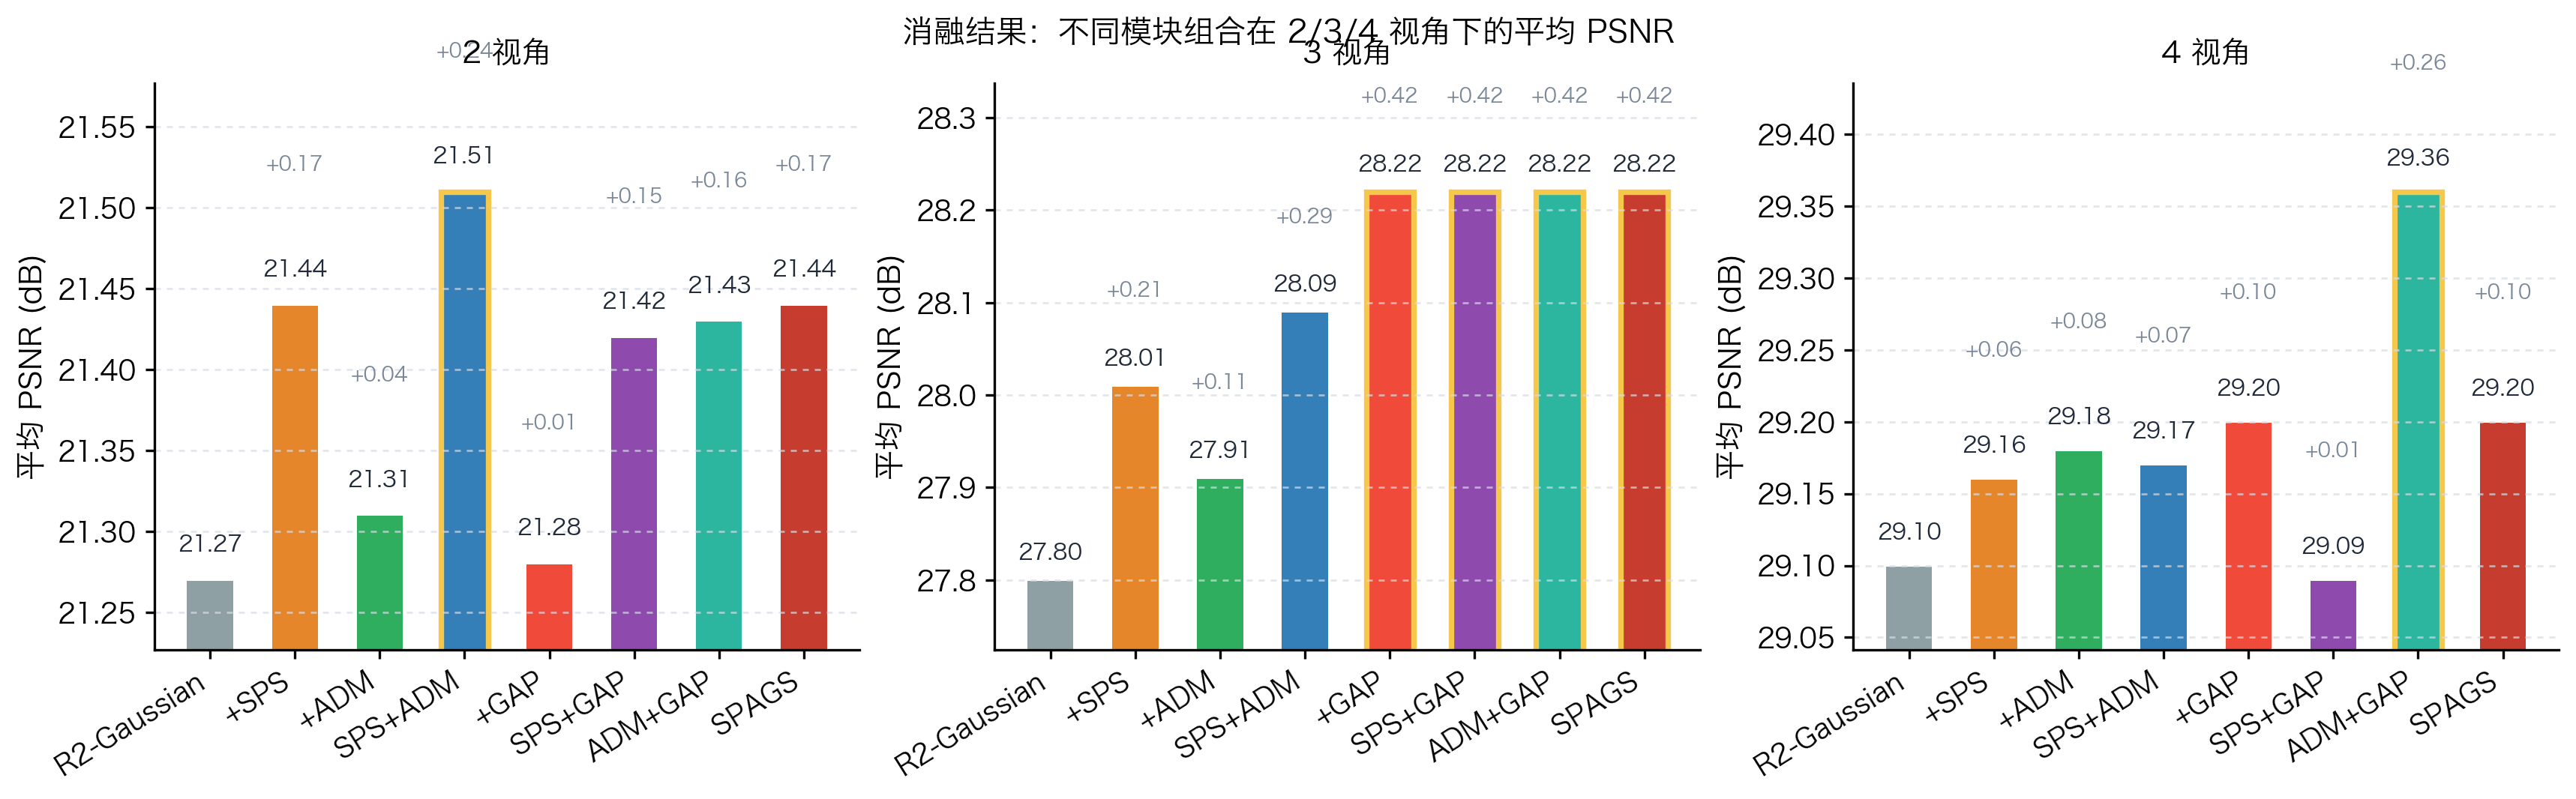
\includegraphics[width=\columnwidth]{figures/fig_ablation_final.png}
\caption{完整消融结果可视化。平均 PSNR 的变化说明，引入 \gap\ 会带来最稳定的性能抬升。}
\label{fig:ablation-chart}
\end{figure}

\subsection{超参数与效率分析}

我们进一步对核心模块进行超参数分析，结果如表~\ref{tab:hyperparams} 所示。整体而言，\sps\ 与 \adm\ 对参数变化较为平滑，而 \gap\ 的阈值对性能更敏感，说明冗余控制强度需要与场景几何复杂度保持平衡。

\begin{table}[t]
\centering
\caption{关键超参数扫描与最终采用值。}
\label{tab:hyperparams}
\small
\renewcommand{\arraystretch}{1.08}
\setlength{\tabcolsep}{3.0pt}
\begin{tabular}{@{}>{\raggedright\arraybackslash}p{0.11\columnwidth}>{\raggedright\arraybackslash}p{0.24\columnwidth}>{\raggedright\arraybackslash}p{0.39\columnwidth}>{\raggedright\arraybackslash}p{0.14\columnwidth}@{}}
\toprule
\textbf{模块} & \textbf{参数} & \textbf{候选值} & \textbf{采用值} \\
\midrule
\sps & uniform ratio & 0.2 / 0.3 / 0.4 & \textbf{0.2} \\
\sps & $\gamma$ & 1.0 / 0.8 / 0.7 & \textbf{1.0} \\
\sps & 初始化策略 & raw / valid mean & \textbf{raw} \\
\sps & 高斯数量 & 50K / 75K & \textbf{50K} \\
\midrule
\gap & 剪枝阈值 $\tau$ & 0.010 / 0.015 / 0.020 & \textbf{0.015} \\
\gap & 最大剪枝比 $\beta$ & 2\% / 3\% / 5\% & \textbf{2\%} \\
\gap & 启动迭代 & 1K / 2K / 5K & \textbf{2K} \\
\gap & 截止迭代 & 15K / 20K / 30K & \textbf{20K} \\
\midrule
\adm & 预热迭代 & 12K / 15K / 18K & \textbf{15K} \\
\adm & 最大调制范围 & 0.2 / 0.3 / 0.4 & \textbf{0.3} \\
\adm & K-Planes 分辨率 & 64 / 128 & \textbf{64} \\
\bottomrule
\end{tabular}
\renewcommand{\arraystretch}{1.0}
\end{table}

\begin{figure}[t]
\centering
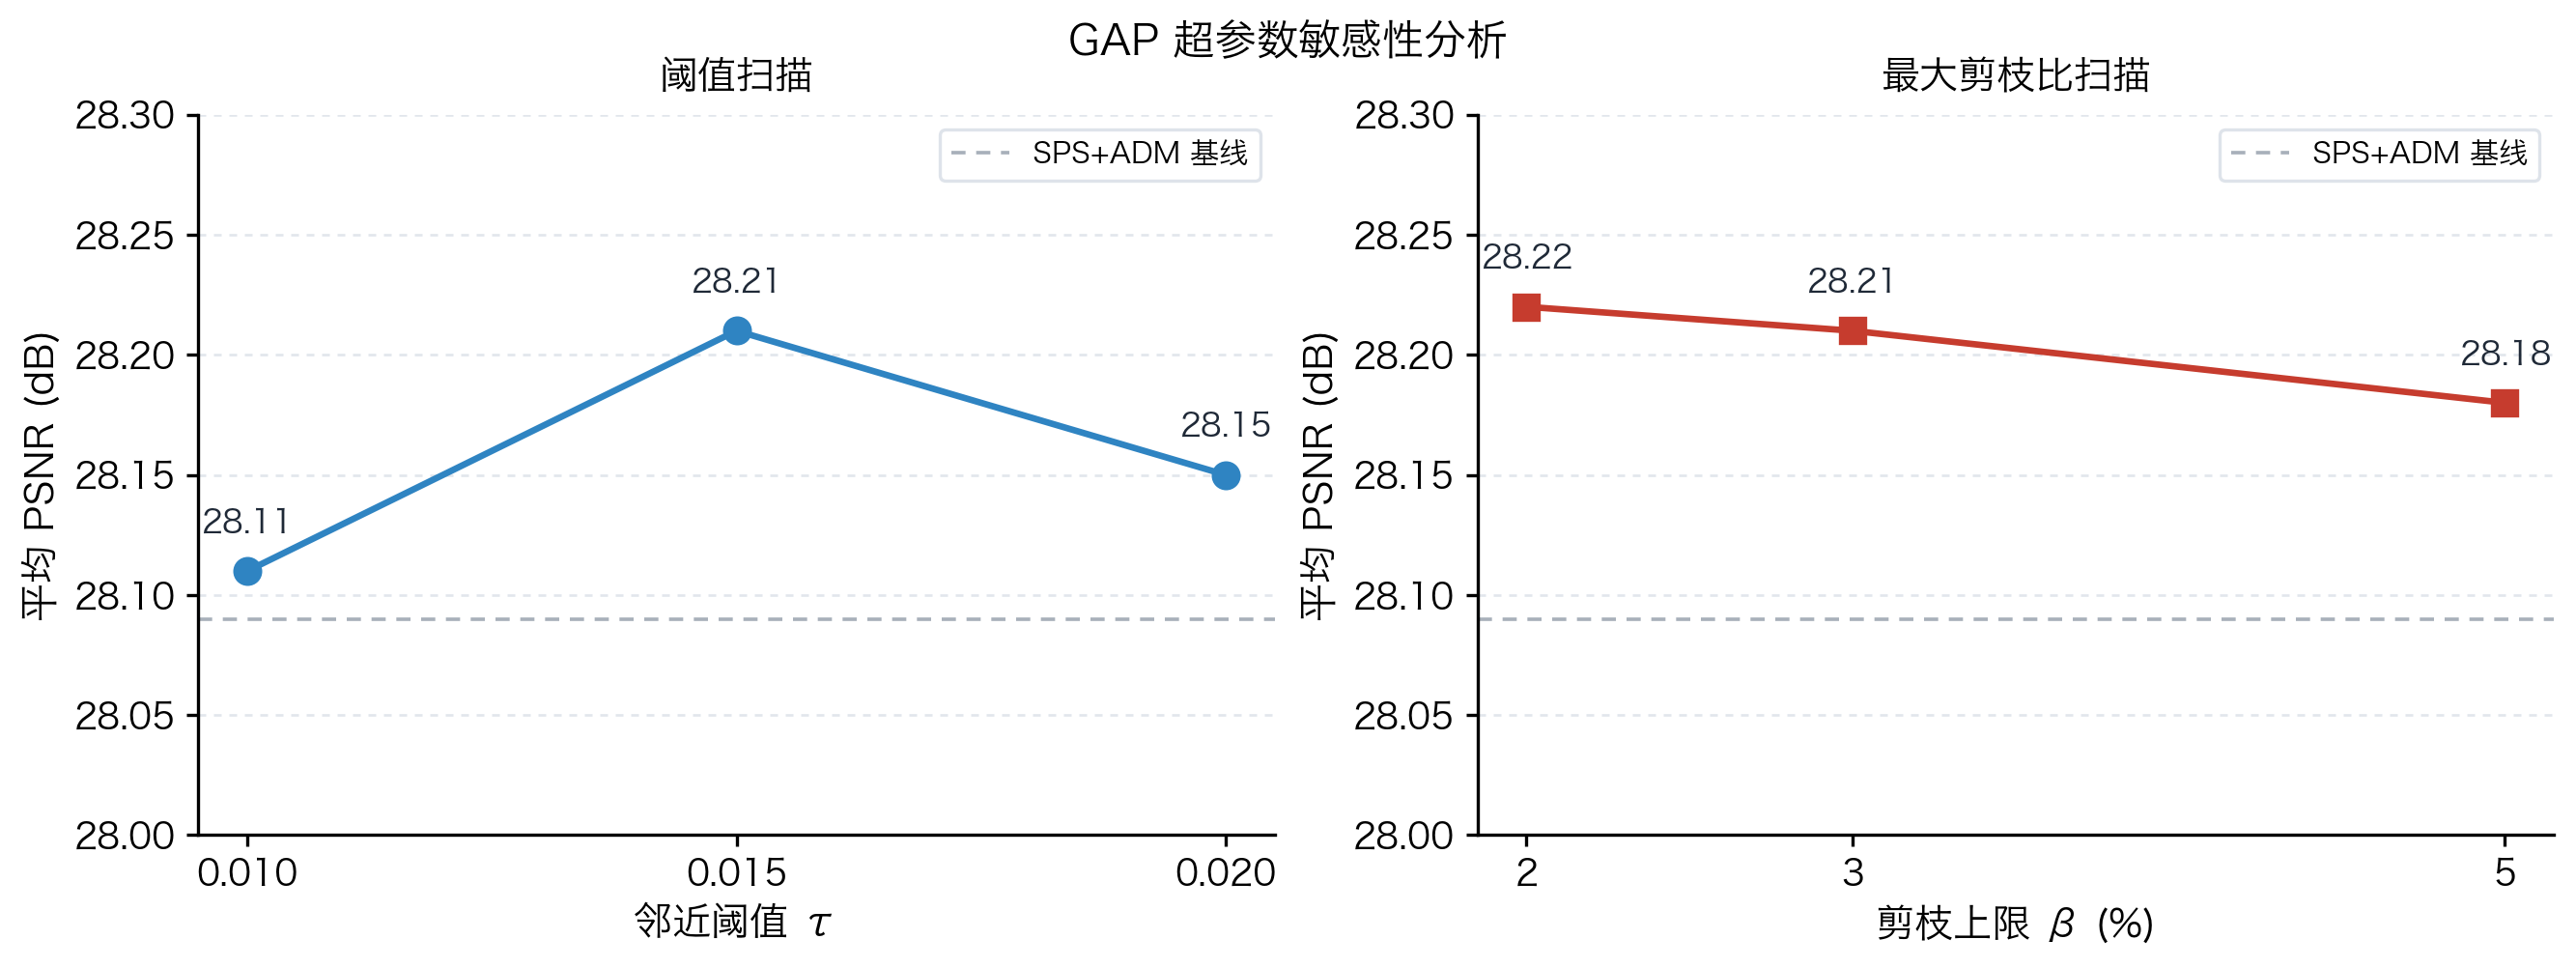
\includegraphics[width=\columnwidth]{figures/fig_gap_sweep.png}
\caption{\gap\ 的阈值与剪枝比扫描。阈值过低时剪枝保守，过高时则会伤害有效高斯。}
\label{fig:gap-sweep}
\end{figure}

效率方面，\sps\ 只在训练前增加一次性的 FDK 预处理；\gap\ 主要开销来自周期性的 KNN 近邻计算；\adm\ 则仅在后半程训练中引入轻量前向与反向传播。整体上，\spags\ 的训练时长仅比 \rtwo\ 高不到 10\%，推理阶段几乎不增加额外负担。考虑到其在 3-view 设定下稳定带来的质量收益，这一成本是可接受的。

\subsection{讨论}

主结果与消融实验共同支持了一个结论：在稀疏视角 CT 场景中，真正决定性能上限的往往不是“是否继续补更多高斯”，而是“能否在空间上把高斯放对位置，并及时移除错误冗余”。这也是为什么 \gap\ 在我们的设定里表现得比 \sps\ 与 \adm\ 更强。另一方面，\sps\ 与 \adm\ 的价值更多体现在为训练过程提供更好的起点和更稳定的密度修正机制，它们让 \gap\ 的剪枝判断更可靠、让最终密度分布更平滑，从而在更广泛的器官与视角设置下保持稳定收益。

\section{结论}
\label{sec:conclusion}

本文提出 \spags，面向稀疏视角 CT 新视图合成，在 3DGS 管线的初始化、密度控制与密度调制三个阶段显式引入空间感知。与已有 sparse-view 3DGS 方法主要围绕补点、深度正则或双场协同不同，我们强调 CT 体数据中的主要矛盾往往是结构冗余而非单纯稀疏，并据此提出 \sps/\gap/\adm\ 三个互补模块。实验结果表明，\spags\ 在 5 个器官、2/3/4 视角设定中取得稳定提升，尤其在最核心的 3-view 条件下，相比 \rtwo\ 获得 0.39 dB 的平均 PSNR 增益。

当前工作仍有若干值得继续推进的方向。首先，\adm\ 的特征分辨率与调制范围目前对不同器官共享，未来可以探索跨器官自适应配置；其次，本文主要评估静态稀疏视角 CT，如何扩展到 cone-beam 或 4DCT 场景仍值得深入研究；最后，若能将病例级优化与更强的学习型体先验结合，\spags\ 还有望在极端稀疏条件下进一步提升稳定性。

\printbibliography
\end{document}
